\section{半间歇釜式反应器}


\begin{frame}
    \frametitle{半间歇操作的适用场合}

    \large \begin{itemize}
        \item 要求一种反应物的浓度高而另一种反应物的浓度低时，采用半间歇操作是有利的。
        \item 需要控制反应温度时，除了通过冷却介质移走热量外，还可采用半间歇操作调节加料速度以控制温度。
        \item 为了提高某些可逆反应的产品收率，可采用半间歇操作，不断移走产物，与此同时还可提高反应过程速率。
    \end{itemize}
    半间歇釜式反应器的设计方程：
    \[
        Q_0c_{i0}=Qc_{i}-\mathcal{R}_iV_\mathrm{r}+\mathrm{d}n_i/\mathrm{d}t \qquad (i=1,2,\cdots,K)
    \]
\end{frame}


\begin{frame}
    \frametitle{半间歇釜式反应器}

    设反应器内进行如下液相反应：
    \[
    \ce{A + B -> R} \qquad r_\mathrm{A}=k'c_\mathrm{A}c_\mathrm{B}
    \]
    \[
        Q_{0} c_{\mathrm{A} 0}=Q c_{\mathrm{A}}-\mathscr{R}_{\mathrm{A}} V+\frac{\mathrm{d}(V c_{\mathrm{A}})}{\mathrm{d} t} 
    \]
    式中$V$为反应器中反应混合物的体积，其值随时间而变。假定操作开始时先向反应器中注入体积为$V_0$的B，然后连续地输入A，流量为$Q_0$，浓度为$c_\mathrm{A0}$，且不连续导出物料，即
    \[
        Q_{0} c_{\mathrm{A} 0}=-\mathscr{R}_{\mathrm{A}} V+\frac{\mathrm{d}(V c_{\mathrm{A}})}{\mathrm{d} t} 
    \]
    又设B大量过剩，则该反应可按一级反应处理
    \[
        \frac{\mathrm{d}(V c_{\mathrm{A}})}{\mathrm{d} t}+k V c_{\mathrm{A}}=Q_{0} c_{\mathrm{A} 0} 
    \]
\end{frame}


\begin{frame}
    \frametitle{半间歇釜式反应器}

    \large 若为恒速加料，任意时间下反应混合物的体积
    \[
        V=V_{0}+Q_{0} t 
    \]
    结合初始条件$t=0$，$V c_{\mathrm{A}}=0$，解该一阶线性微分方程得
    \begin{columns}[c]
        \column{7cm}
        \[
        V c_{\mathrm{A}}=\frac{Q_{0} c_{\mathrm{A} 0}}{k}[1-\exp (-k t)] 
    \]
    \[
        \frac{c_{\mathrm{A}}}{c_{\mathrm{A} 0}}=\frac{1-\exp (-k t)}{k(t+V_{0} / Q_{0})}
    \]
        \column{6.5cm}
        \[
            V c_{\mathrm{R}}=Q_{0} c_{\mathrm{A} 0} t-V c_{\mathrm{A}} 
        \]
        \[
            \frac{c_{\mathrm{R}}}{c_{\mathrm{A} 0}}=\frac{k t-[1-\exp (-k t)]}{k(t+V_{0} / Q_{0})}
        \]
    \end{columns}
    
    

\end{frame}


\begin{frame}
    \frametitle{半间歇釜式反应器}

    \begin{columns}[c]
        \column{7.8cm}
       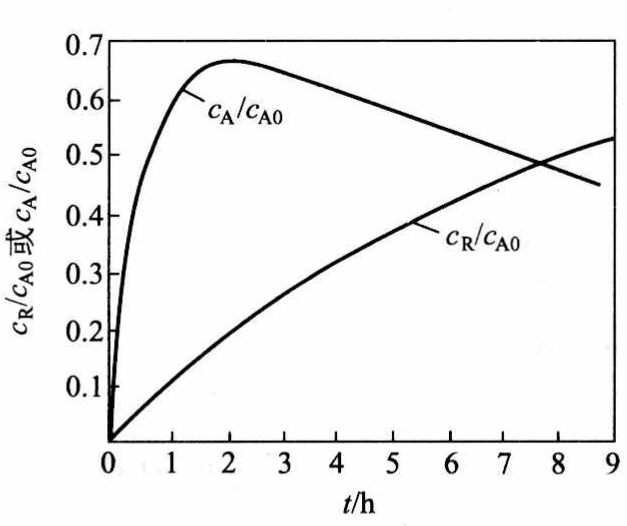
\includegraphics[width=\linewidth]{figs/fig3.12.png}
        \column{5.7cm}
        当$k=0.2\mathrm{h^{-1}}$，$V_0/Q_0=0.5\mathrm{h}$时，半间歇釜式反应器内反应组分浓度与时间的关系如图所示。
        \begin{itemize}
            \item[\bullet] 反应物A的浓度与时间的关系曲线存在一极大值
            \item[\bullet] 反应产物R的浓度总是随反应时间的增加而增加
        \end{itemize}
    \end{columns}

\end{frame}


\begin{frame}[t]
    \frametitle{}

    \begin{example}
        在等温间歇釜式反应器中进行下列液相反应
        \[
            \ce{A + B -> P} \qquad r_\mathrm{P}=2c_\mathrm{A} \quad \si{kmol.m^{-3}.h^{-1}}
        \]
        \[
            \ce{2A -> Q} \qquad r_\mathrm{Q}=0.5c_\mathrm{A}^2 \quad \si{kmol.m^{-3}.h^{-1}}
        \]
        先把\SI{1}{m^3}浓度为\SI{4}{kmol/m^3}的B放入釜内，然后将\SI{1}{m^3}浓度为\SI{4}{kmol/m^3}的A于\SI{3}{h}内连续均匀地加入，使之与B反应。试问A加完时，组分A和P的浓度各为多少？

    \end{example}

\end{frame}